% Ausgelagert %

% =========================================================================== %

\begin{frame}[t,fragile]%{\mintinline{c}{static} -- residente Variablen}
%
\begin{columns}[T]
\column{.3\linewidth}
\begin{Large}
\mintinline{c}{static} -- residente Variablen
\vspace{10pt}
\end{Large}
\begin{itemize}
\item Modifier \mintinline{c}{static} \emph{vor} Datentyp
\item Wert einer Variablen ändert sich zwischen zwei Funktionsaufrufen nicht
\item Ändert nichts an Sichtbarkeit (Scopes)
\item Optionaler Startwert wird nur ein einziges Mal zugewiesen
\end{itemize}
%
\column{.7\linewidth}
\begin{codebox}[Beispiel]
\begin{minted}[fontsize=\scriptsize, linenos]{c}
#include <stdio.h>

void recursive (int maxDepth) {
   static int current = 0;
   int i;
   printf("Entry into 'recursive' at depth %d\n", current);

   if (current < maxDepth) {
      current++;
      for (i=0; i<current; i++) {printf(" ");}
      recursive(maxDepth);
   }

   for (i=0; i<current; i++) {printf(" ");}
   printf("Leaving 'recursive' at depth %d\n", current);
   current--;
}

int main(void) {recursive(5);}
\end{minted}
\end{codebox}
\end{columns}

%
\end{frame}

% =========================================================================== %

\begin{frame}[t]{Code-Strukturierung: Beispiel Matrix-Multiplikation}
%
\begin{columns}[T]
\column{.5\linewidth}
\begin{itemize}
\item Aufgabe: Komplexwertige Matrixmultiplikation
\item Herangehen:
	\begin{itemize}
	\item Hauptprogramm: zwei Matrizen
	\item Unterprogramm 1: Matrix-Multiplikation
	\item Unterprogramm 2: Multiplikation komplexer Zahlen
	\item[$\Rightarrow$] Erstes Unterprogramm ruft zweites Unterprogramm auf!
	\end{itemize}
\end{itemize}
%
\column{.5\linewidth}
\begin{itemize}
\item Kein Limit für Verschachtelung
\item Tradeoff: Geschwindigkeit vs. Lesbarkeit
\item Häufig: Routinen \enquote{wiederverwendbar}!
\end{itemize}
%
\vspace{10pt}
\begin{adjustbox}{max totalsize={.9\textwidth}{.7\textheight},center}
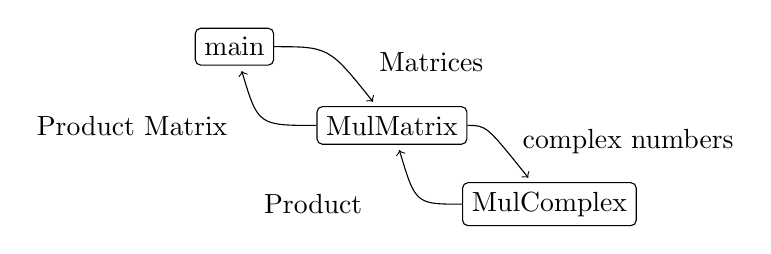
\begin{tikzpicture}[
  proc/.style={shape=rectangle,draw=black,rounded corners=2pt},
  flow/.style={draw=black,->,shorten >=2pt}
]
  \node[proc] (main)       at (0,2) {main};
  \node[proc] (MulMatrix)  at (2,1) {MulMatrix};
  \node[proc] (MulComplex) at (4,0) {MulComplex};
  
  \draw[flow] (main) .. controls +(1.2,0) .. (MulMatrix);
  \node at (2.5,1.8) {Matrices};
  
  \draw[flow] (MulMatrix) .. controls +(-1.7,0) .. (main);
  \node at (-1.3,1) {Product Matrix};
  
  \draw[flow] (MulMatrix) .. controls +(1.2,0) .. (MulComplex);
  \node at (5,0.8) {complex numbers};
  
  \draw[flow] (MulComplex) .. controls +(-1.7,0) .. (MulMatrix);
  \node at (1,0) {Product};
\end{tikzpicture}
\end{adjustbox}
%
\end{columns}
%
\begin{hintbox}
Fluss-Skizzen anlegen!
\end{hintbox}
%
\end{frame}